\begin{figure}[htbp]
\centering
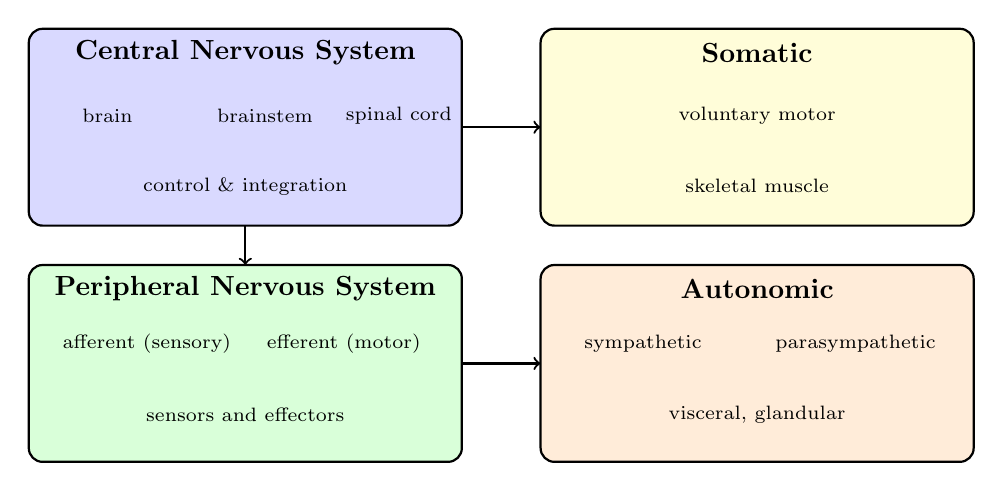
\begin{tikzpicture}[scale=1.0, every node/.style={font=\small}]
  % CNS box
  \draw[thick, fill=blue!15, rounded corners=5pt] (0,3) rectangle (5.5,5.5);
  \node[font=\bfseries] at (2.75,5.2) {Central Nervous System};
  \node[align=center, font=\scriptsize] at (1.0,4.4) {brain};
  \node[align=center, font=\scriptsize] at (3.0,4.4) {brainstem};
  \node[align=center, font=\scriptsize] at (4.7,4.4) {spinal cord};
  \node[align=center, font=\scriptsize] at (2.75,3.5) {control \& integration};
  % PNS box
  \draw[thick, fill=green!15, rounded corners=5pt] (0,0) rectangle (5.5,2.5);
  \node[font=\bfseries] at (2.75,2.2) {Peripheral Nervous System};
  \node[align=center, font=\scriptsize] at (1.5,1.5) {afferent (sensory)};
  \node[align=center, font=\scriptsize] at (4.0,1.5) {efferent (motor)};
  \node[align=center, font=\scriptsize] at (2.75,0.6) {sensors and effectors};
  % Autonomic box
  \draw[thick, fill=orange!15, rounded corners=5pt] (6.5,0) rectangle (12,2.5);
  \node[font=\bfseries] at (9.25,2.2) {Autonomic};
  \node[align=center, font=\scriptsize] at (7.8,1.5) {sympathetic};
  \node[align=center, font=\scriptsize] at (10.5,1.5) {parasympathetic};
  \node[align=center, font=\scriptsize] at (9.25,0.6) {visceral, glandular};
  % Somatic label
  \draw[thick, fill=yellow!15, rounded corners=5pt] (6.5,3) rectangle (12,5.5);
  \node[font=\bfseries] at (9.25,5.2) {Somatic};
  \node[align=center, font=\scriptsize] at (9.25,4.4) {voluntary motor};
  \node[align=center, font=\scriptsize] at (9.25,3.5) {skeletal muscle};
  % Arrows
  \draw[->, thick] (2.75,3) -- (2.75,2.5);
  \draw[->, thick] (5.5,1.25) -- (6.5,1.25);
  \draw[->, thick] (5.5,4.25) -- (6.5,4.25);
\end{tikzpicture}
\caption[Nervous system hierarchy]{The vertebrate nervous system at a
glance. The central nervous system (brain and spinal cord) integrates
sensory input and issues motor commands. The peripheral nervous system
carries information between the CNS and the body, with somatic
(voluntary) and autonomic (involuntary) branches; the autonomic
divides into sympathetic and parasympathetic arms.}
\label{fig:vol06:ch07:ns-hierarchy}
\end{figure}
